\chapter{Экспериментальная часть}
В этом разделе будет продемонстрирована работа программы, а также
приведены результаты тестирования алгоритмов.

\section{Демонстрация работы программы}
На рисунке 4.1 приведена демонстрация работы программы.

\FloatBarrier
\begin{figure}[h]
	\begin{center}
		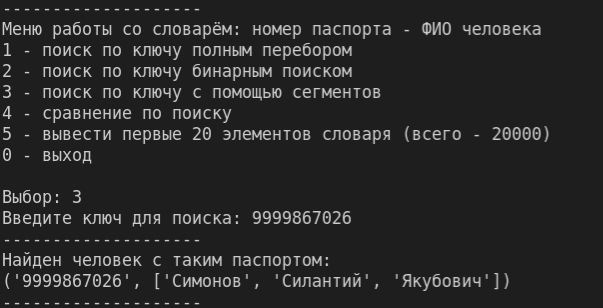
\includegraphics[]{inc/demostrate.jpg}
	\end{center}
	\caption{Демонстрация работы программы}
\end{figure}
\FloatBarrier

\section{Технические характеристики}
Технические характеристики устройства, на котором выполнялось тестирование, следующие:
\begin{itemize}
	\item операционная система: Windows 10;
	\item память: 8 GB;
	\item процессор: Intel Core i5-1135G7 @ 2.40GHz \cite{intel}.
\end{itemize}

Во время тестирования ноутбук был нагружен только встроенными приложениями окружения, а также непосредственно системой тестирования.

\section{Тестирование программы}
Для определения быстродействия работы алгоритмов будет проведено исследование зависимости
на квадратных матрицах, так как её размер однозначно определяется по одной переменной. 
По оси X будет откладываться размер квадратной матрицы, а по оси Y - время работы алгоритмов
в наносекундах.

\subsection{Тестирование работы алгоритмов при чётном размере матрицы}
В таблице 4.1 представлены результаты тестирования времени работы алгоритмов при чётном размере
квадратной матрицы.

\FloatBarrier
\begin{table}[h]
	\caption{Результаты тестов для чётных размеров матрицы}
	\centering
	\begin{tabular}{ | l | l | l | l |}
		\hline
		Размер массива & Classic & Vinograd & optVinograd \\ \hline
		2 & 31250 & 31250 & 32500 \\
		4 & 156250 & 187500 & 218750 \\
		6 & 468750 & 625000 & 500000 \\
		10 & 1687500 & 1625000 &  1781250 \\
		16 & 10750000 & 19562500 & 18875000 \\
		30 & 110416666 & 107291666 & 104166666 \\
		50 & 569791666 & 554166666 & 489583333 \\
		76 & 1816666666 & 1694791666 & 1576041666 \\
		100 & 4309375000 & 4093750000 & 3835416666 \\
		200 & 33953125000 & 33484375000 & 32640625000 \\
		400 & 218296875000 & 91078125000 & 81812500000 \\
		\hline
	\end{tabular}
\end{table}
\FloatBarrier

На рисунке 4.2 изображён график зависимости времени работы алгоритмов от размера 
квадратной матрицы при чётных размерах матрицы.

\FloatBarrier
\begin{figure}[h]
	\begin{center}
		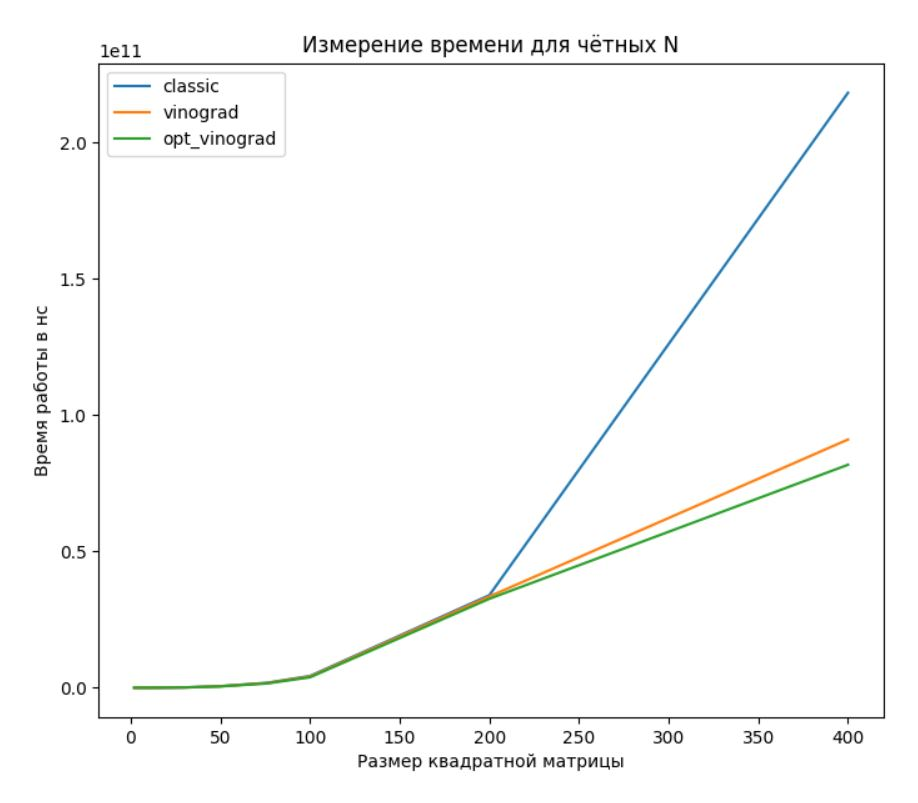
\includegraphics[width=\linewidth]{inc/chet.jpg}
	\end{center}
	\caption{График зависимости времени работы алгоритмов умножения на матрицах чётных размеров}
\end{figure}
\FloatBarrier

\subsection{Тестирование работы алгоритмов при нечётном размере матрицы}
В таблице 4.2 представлены результаты тестирования времени работы алгоритмов при нечётном размере
квадратной матрицы.

\FloatBarrier
\begin{table}[h]
	\caption{Результаты тестов для нечётных размеров матрицы}
	\centering
	\begin{tabular}{ | l | l | l | l |}
		\hline
		Размер массива & Classic & Vinograd & optVinograd \\ \hline
		1 & & 52083 & \\
		3 & 104166 & 104166 & 4687 \\
		5 & 208333 & 312500 & 260416 \\
		9 & 1302083 & 1250000 &  1145833 \\
		15 & 5416666 & 5208333 & 5572916 \\
		31 & 41666666 & 48958333 & 107291666 \\
		51 & 448958333 & 192708333 & 197916666 \\
		75 & 626041666 & 609375000 & 577083333 \\
		101 & 1637500000 & 1675000000 & 1531250000 \\
		201 & 11859375000 & 10640625000 & 10140625000 \\
		401 & 91437500000 & 87062500000 & 81265625000 \\
		\hline
	\end{tabular}
\end{table}
\FloatBarrier

На рисунке 4.3 изображён график зависимости времени работы алгоритмов от размера 
квадратной матрицы при нечётных размерах матрицы.

\FloatBarrier
\begin{figure}[h]
	\begin{center}
		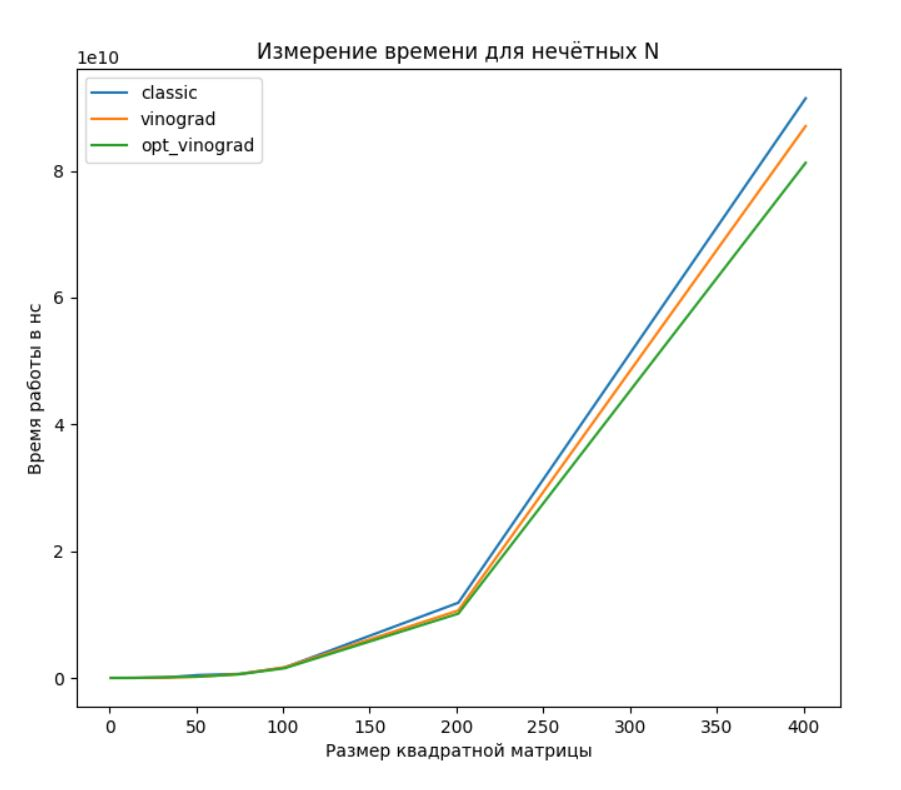
\includegraphics[width=\linewidth]{inc/nechet.jpg}
	\end{center}
	\caption{График зависимости времени работы алгоритмов умножения на матрицах нечётных размеров}
\end{figure}
\FloatBarrier

\section{Вывод}
Было реализовано работающее ПО, реализующее три алгоритма умножения матриц.
Было проведено исследование зависимости работы алгоритмов от размера квадратной матрицы.

Подтвердилось, что у всех алгоритмов один и тот же порядок зависимости, 
что и было предположено в оценке трудоёмкости работы.

На чётных размерах матрицы алгоритмы Винограда сработали быстрее, чем классический алгоритм.
На размере $N=400$ оба алгоритма Винограда работают в два раза быстрее. При этом оптимизированный
алгоритм сработал на 2.5\% быстрее.

На нечётных размерах матрицы алгоритмы Винограла показали более быструю работу.
На размере $N=401$ оптимизированный алгоритм Винограда работал на 7\%, чем обычный Виноград, 
и на 11\% -- чем классический алгоритм. Для $N=201$ аналогичные пропорции составили 
5.5\% и 14\% соответственно.

При этом при значения $N<6$ классический алгоритм работает быстрее, чем алгоритм Винограда,
и для маленьких матриц такие преобразования не имеют смысл.

По затратам памяти классический алгоритм имеет зависимость $O(1)$, а алгоритмы Винограда -- $O(N)$.
Это связано с тем, что в алгоритмах Винограда изначально сохраняются значения в массивы. 
